\documentclass{life-fr}

\begin{document}

\title{La Vie est un Jeu}
\subtitle{Documentation Utilisateur}
\member{Lepage Barbara}{lepage.barbara@gmail.com}
\member{Caradec Guillaume}{guillaume.caradec@gmail.com }
\member{Corsin Simon}{simoncorsin@gmail.com }
\member{Glorieux François}{fra.glorieux@gmail.com}
\member{Klarman Nicolas}{nickoas@gmail.com}
\member{Lassagne David}{david.lassagne@gmail.com}
\member{Louvigny Guillaume}{guillaume@louvigny.fr}
\member{El-Outmani Youssef}{youssef.eloutmani@gmail.com}
\member{Le-Cor Wilfried}{wilfried.lecor@gmail.com}
\member{Lenormand Frank}{lenormf@gmail.com}

\summary
{
	Ce document présente le projet « La Vie Est Un Jeu » du point de vue de l'utilisateur final.
}

\maketitle
\authorspage

%% --------------------------------------------------------------------- %%

\chapter*{Résumé}
{
	«~La Vie Est Un Jeu~» est un projet sur trois ans dans le cadre des «~Epitech
	Innovative Projects~» mené par un groupe de dix étudiants.\\
	\\
	Ce projet, sous forme d'un site web et d'applications mobiles, propose à
	ses utilisateurs de pimenter leur quotidien. Pour cela, on leur propose
	de manière ludique de se fixer des objectifs, les réaliser, les collectionner
	et enfin les partager.\\
	C'est donc à la fois un jeu et un réseau social, destiné à tous les âges !\\
	\\

	Dans ce document traitant de l'utilisation de notre projet, nous nous efforcerons d'avoir une approche aussi globale que possible sur les fonctionnalités et attentes des utilisateurs.
}

\chapter*{Informations du document}

\rowcolors{1}{white}{lightgray}
\begin{tabular}{ | m{5cm} | m{10cm} | }
	\hline
	\textbf{Type du document} & Documentation Utilisateur\\ % to change
	\hline
	\textbf{Titre complet du document} & Documentation Utilisateur du projet «~La Vie Est Un Jeu~»\\ % to change
	\hline
	\textbf{Mots clés} & «~Utilisateur~», «~Tutoriel~», «~conception~», «~lavieestunjeu~»\\ % to change
	\hline
	\textbf{Nombre de pages} & \ref{TotPages} \\
	\hline
	\textbf{Nom du groupe} & La Vie Est Un Jeu\\
	\hline
	\textbf{Responsable} & Chef de groupe : Barbara Lepage\\
	\hline
	\textbf{Membres du groupe} & Voir page de garde\\
	\hline
	\textbf{Auteurs} & Membres du groupe, voir page de garde\\
	\hline
	\textbf{Contact} & lavieestunjeu@googlegroups.com\\
	\hline
	\textbf{Révision actuelle} & 1.0\\ % to change
	\hline
	\textbf{Site vitrine} & \url{http://eip.epitech.eu/2014/lavieestunjeu/}\\
	\hline
	\textbf{Site officiel} & Non disponible\\
	\hline
\end{tabular}

\newpage

\tableofcontents

%% --------------------------------------------------------------------- %%

\chapter{Introduction et contexte}

\section{«~La Vie Est Un Jeu~»}

\subsection{«~La vie est un Jeu~», bien plus qu'un simple réseau social !}

À l'instar de plusieurs solutions déjà existante, nous avons l'ambition de créer un reseau social mais en apportant notre propre vision.
Celui ci comportera donc un parcours à but ludique basé sur les «~listes de choses à faire avant de mourir~» : il définit toutes les choses que vous désirez faire de vôtre existence, une sorte de mémo pour vous rappeller vos accomplissements. Notre projet vous permettra de construire vôtre propre liste et de faire valider vos exploits tout en les partageant avec les personnes/entités présentes dans vos contacts. Ainsi, chaque action réalisée par un utilisateur (ajout d'une activité, succès ou échec) sera un fil de discussion dans lequel le visiteur et son réseau pourront discuter et partager différents types de médias (photos, vidéos, etc.). Ce fil de discussion se trouvera sur les flux d'informations propres à chacun. L'activité d'un utilisateur sera validée par son propre réseau et apparaîtra sous forme de «~succès~», comme dans un jeu vidéo. Le site s'étendra par la suite en proposant d'autres caractéristiques propres aux jeux vidéo.\\
\\
Ce côté novateur ne nous semblait pas assez ou peu exploité, voici donc une occasion pour vous, fans de défis, de garder une trace des actions et rencontrer des gens qui partagent peut-être la même passion que vous !

%% --------------------------------------------------------------------- %%

\section{Vocabulaire du projet}

\subsection{Qu'est-ce qu'un «~achievement~» ?}
Le terme achievement (qui peut être traduit par succès ou réalisation en français) est, dans le cadre vidéoludique,  un objectif défini à accomplir par le joueur, en dehors de l’objectif principal (c’est-à-dire, gagner ou finir le jeu).\\
 Les achievements sont donc des récompenses honorifiques ajoutant du challenge pour le joueur.\\
\\
Nous pourrions utiliser une traduction française du terme achievement mais nous pensons que achievement est le terme le plus populaire dans le monde vidéoludique.\\
\\
Les achievements permettent au joueur de découvrir plus en profondeur le contenu du jeu et donc d’explorer de nouveaux horizons.\\
 L’obtention est souvent un moment agréable pour le joueur.\\
 Il ressent une certaine satisfaction et se sent récompensé pour un effort.\\
 Il peut ensuite les partager avec ses amis afin de recueillir les honneurs ou défier ses amis de faire autant ou mieux, ce qui améliore grandement l’immersion au sein du jeu.\\
\\
Nous pensons, qu’il est intéressant d’en faire une analogie avec la vie.\\
 La vie est un jeu comme un autre et mérite d’avoir elle aussi ses achievements.

 Nous avons noté chez les solutions existantes un certain manque d'accentuation sur les centre d'intérets et c'est pour cela qu'au fur et à mesure qu'un utilisateur valide des achievements, son profil sera de plus en plus identifiable comme étant intéressant pour d'autres personnes. Ceci dans le but de les amener naturellement à se regrouper selon les passions de chacun.

\subsection{Définitions, Acronymes et Abréviations}

\begin{description}
\item[Achievement]
Récompense suite à une ou plusieurs actions.

\item[Application mobile]
Une application mobile est une application développée pour être installée sur un appareil électronique mobile.

\item[Login]
En français «~Identifiant~», c'est une information permettant à une personne de s'identifier auprès d'un système.

\item[Réseau social]
Ensemble d'identités sociales, telles que des individus ou encore des organisations, reliées entre elles par des liens créés lors d’interactions sociales.

\item[Smartphone]
Téléphone mobile disposant aussi des fonctions d'un assistant numérique personnel. Il fournit des fonctionnalités basiques comme l'agenda, le calendrier, la navigation sur le Web, la consultation du courrier électronique, la messagerie instantanée, le GPS, ...

\item[Android]
Système d’exploitation utilisant le noyau Linux pour smartphones, PDA et terminaux mobiles conçu par Android, une startup rachetée par Google.

\item[iOS]
Système d’exploitation mobile développé par Apple pour l'iPhone, l'iPod touch, et l'iPad. Il est dérivé de Mac OS X dont il partage les fondations.

\item[Windows Phone]
Système d’exploitation mobile développé par Microsoft pour succéder à Windows Mobile, sa précédente plate-forme logicielle.

\item[Version Bêta]
Version de test comportant toutes les fonctionnalités d'un programme. C'est grâce à cette version que les testeurs remontent les éventuels problèmes.

\item[Wiki]
Espace collaboratif sur lequel les utilisateurs sont invités à rédiger des documents de travail.


\end{description}


%% --------------------------------------------------------------------- %%

\subsection{But final du projet}

Le projet a pour but de créer une communauté d'utilisateurs autour d'un système d'achievements, directement lié à la vie quotidienne, aux passions ou à la vie professionnelle, ceci dans le but de vous permettre de trouver des gens qui partagent éventuellement des passions et intérets communs avec vous.\\

Vous êtes très nombreux ! En théorie, toute personne ayant un centre d'interêt ou une passion est une cible.\\

À plus long terme, des partenariats commerciaux permettront de cibler des marques et des lieux.\\

Le site sera multilingue, donc ouvert à l'internationalisation.

% --------------------------------------------------------------------- %%

\chapter{Description des différentes parties des services internet et mobiles}

\section{Le site web}

\subsection{Vue d'ensemble de la page d'accueil avant le login}

Vous verrez en premier lieu un diaporama mettant en avant certains achievements, classés par date de publication et par popularité, ainsi que les diverses fonctions du site. Ce diaporama a pour but de vous inciter à procéder à son inscription de manière ludique.\\

La page d'accueil permettra également de s'inscrire au site. Cette inscription est détaillée plus loin.\\

La dernière fonctionnalité principale de cette page d'accueil est vôtre connexion au site.\\

L'entrée du site pourrait éventuellement permettre de rechercher les achievements et catégories de celui-ci.

\newpage

\subsection{L'inscription, les cinq premières minutes !}

L'objectif de cette étape serait clairement d'éviter toute la lourdeur que représente la récolte d'informations que le site a besoin d'effectuer auprès de vous
(présenter un formulaire compact et sauvage a des chances de rebuter celui-ci et éventuellement de vous faire renoncer à l'inscription).\\

Nous avons donc pensé à un système en mode pas à pas qui, tout en faisant découvrir notre outil et son univers à l'internaute, effectuerait de subtiles demandes d'informations de façon régulière, et ce afin d'alléger cette étape essentielle qui nous permettra de catégoriser le nouvel inscrit et de lui proposer du contenu en fonction de ces informations qui auront été récoltées.\\

En plus de combiner le rôle de « guide » pour la découverte du site et de « sondeur » pour la récolte d'informations, cette méthode a pour avantage de vous encourager à aller au bout de la présentation et donc de l'inscription (il y a là un effet psychologique, il veut finir ce qu'il a commencé ; puisqu'il a déjà commencé à contribuer, autant aller jusqu'au bout). La présentation allant, l'intérêt croissant, les chances d'une inscription réussie augmentent à l'arrivée.\\
\\

Dans l'état actuel on imagine comme première approche une question simple qui amène à faire une simple action en mode « vous êtes à un clic de rentrer dans notre univers » avec, par exemple, le choix du genre : Homme, Femme, Non précisé.

\begin{figure}[H]
	\begin{center}
		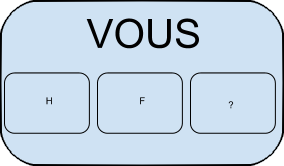
\includegraphics[width=10cm]{img/vous.png}
	\end{center}
\end{figure}

\subsection{La page d'accueil utilisateur une fois connecté}

La page d'accueil de l'utilisateur habitué au site présente son flux d'informations, à l'image des flux habituels de sites communautaires tels que Facebook ou Google+. \\

Le menu est discret, ce qui vous permet de tout de suite voir les quatre onglets principaux :

\begin{itemize}
	\item le flux (page d'accueil par défaut) ;
	\item les objectifs de l'utilisateur (ses inscriptions) ;
	\item les achievements ;
	\item les « amis » de l'utilisateur (importés des réseaux sociaux ou ajoutables dans le cadre du site).
\end{itemize}

Une barre de « breaking news » en permanence en haut du site vous donnera en une ligne les derniers achievements de vos amis ainsi que les nouveautés du site.

\begin{figure}[H]
	\begin{center}
		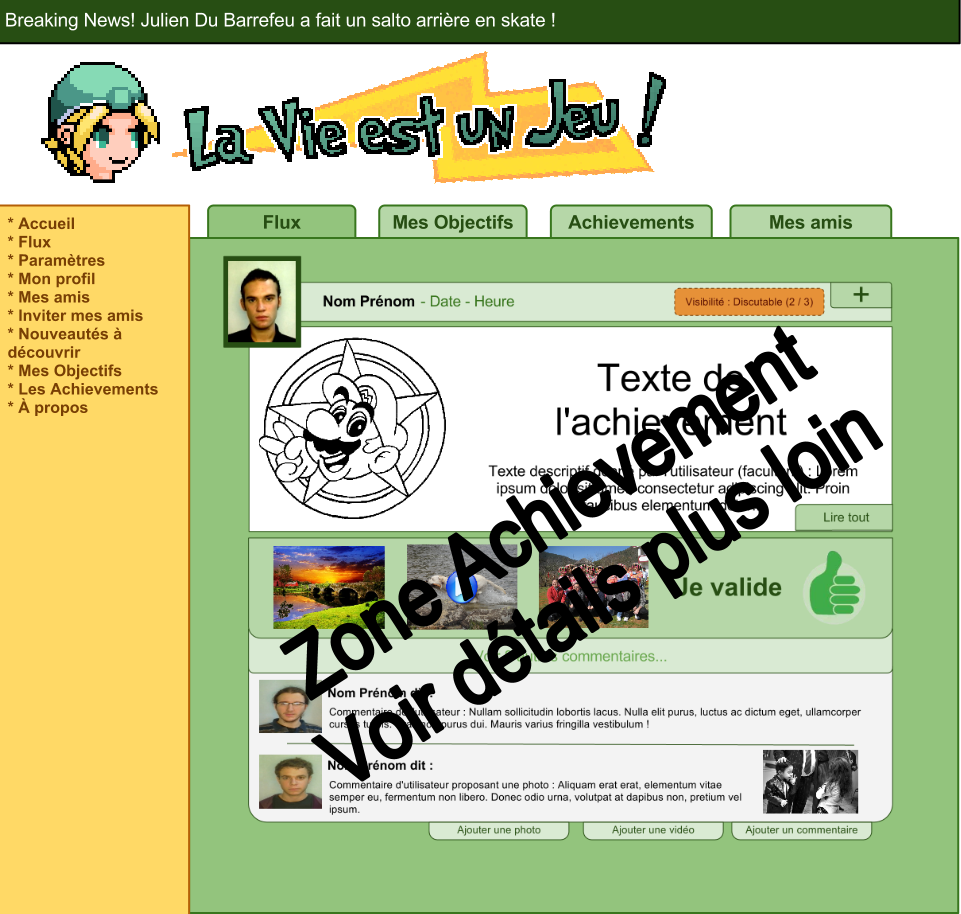
\includegraphics[width=15cm]{img/accueil.png}
	\end{center}
\end{figure}


\subsection{Onglet Flux}

L'onglet Flux sera situé au milieu de la page principale et aura pour fonction d'afficher les derniers achievements réalisés par le réseau social et à valider par le cercle d'amis.\\

Ce flux contiendra toutes les actions des contacts :

\begin{itemize}
	\item les « achievements » à valider (voir détails ci-dessous) ;
	\item les objectifs qu'ils se sont fixés ;
	\item les nouveaux contacts ;
	\item des nouveautés du site (informations ou nouveaux achievements).
\end{itemize}

\newpage

\subsection{Onglet Achievements}

Via cette page, vous pourrez sélectionner des packs qui contiendront les achievements à accomplir. Les packs seront tous disponibles et classés par thématiques dans une sous-catégorie, mais la plate-forme proposera d'abord des packs d'achievements correspondant à vos centres d'intérêt, ou encore à vôtre tranche d'âge. Une fois un pack sélectionné, vous pouvez aussi définir certains achievements comme étant vos objectifs et ainsi notifier vôtre réseau.

\subsection{Détails d'un achievement}

Chaque achievement disposera d'une fonction de validation à l'image des boutons « J'aime » de Facebook ou « +1 » de Google+. Elle permettra aux utilisateurs d'indiquer qu'ils valident la publication en question. Aussi bien le support de validation que les simples commentaires pourront être au format texte, photo et/ou vidéo. La photo (ou « avatar ») de l'utilisateur apparaîtra ainsi que la description de l'achievement, en regard de celle-ci. Il sera également possible de poster des commentaires en-dessous des preuves de validation. Un onglet « Plus » permettra de dérouler chaque achievement afin d'obtenir plus d'informations.\\

\begin{figure}[H]
	\begin{center}
		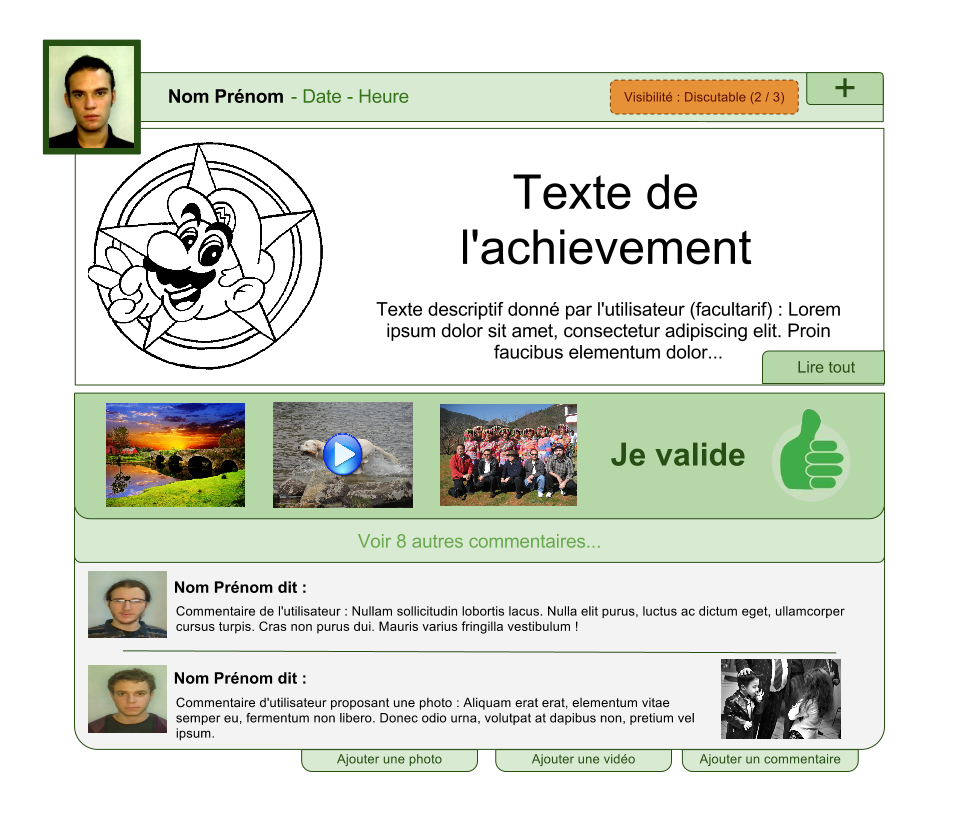
\includegraphics[width=15cm]{img/achievement.png}
	\end{center}
\end{figure}

\subsection{Onglet Objectifs}

L'onglet Objectifs permet à l'utilisateur de construire une liste d'objectifs du quotidien ou de choses à faire absolument avant de mourir. Le but est de filtrer les achievements que l'utilisateur ne désire pas réaliser dans l'immédiat et ainsi de mettre en valeur ceux qu'il va accomplir sur le court terme. La page est destinée à être régulièrement consultée : c'est à partir de cet onglet que l'utilisateur peut annoncer la fin d'un objectif et donc obtenir un achievement si ses amis confirment la validation de ce dernier.

\subsection{Onglet Contacts}

L'utilisateur pourra ici voir sa liste de contacts et les profils de ceux-ci, mais également regrouper ses contacts par groupe. Les groupes d'utilisateurs permettent alors d'attribuer des degrés de sensibilité.\\
Le degré de sensibilité va de 0 à 3 et permet de partager les achievements aux contacts de son choix. Cette fonctionnalité est décrite plus en détails dans la suite du document.

\subsection{Onglet Groupes}

L'utilisateur pourra rejoindre et lister les différents groupes (si ceux-ci sont publics). Ces groupes sont voués à regrouper des achievements, médias ainsi que diverse publications appartenant à la même catégorie ou destinés à être consultés par le même groupe de personnes.

Ainsi cela vous permettra d'accéder à des listes d'achievements supplémentaires mais aussi de contribuer en proposant de nouveaux défis ou simplement en donnant vôtre avis sur ceux déjà présents pour ce groupe.

L'utilisateur a aussi la possibilité de demander à rejoindre la deuxième catégorie d'utilisateur qui est présente dans les groupes, il s'agit des modérateurs : Ils sont en charge de :

\begin{itemize}
\item Vérifier que le comportement des personnes appartenant au groupe est conforme à ce qui est attendu de leur part par le fondateur du groupe.
\item Valider/Invalider les différentes propositions des utilisateurs en terme de publications/achievements
\item Éventuellement rajouter du contenu directement
\end{itemize}

Vient ensuite la dernière catégorie d'utilisateur pour les groupes, le fondateur. Il est gérant du groupe et peut nommer des modérateurs afin de déléguer une partie des responsabilités en terme de gestion du contenu. \\ 

Si vous ne trouvez pas un groupe qui correspond à vos attentes, n'hésitez pas à creer le vôtre cela sera surement utile pour d'autres personnes.

\subsection{Page Profil}

La page Profil contient les informations d'un utilisateur et permet de les modifier. Si l'utilisateur consulte la page profil d'un autre membre, il a la possibilité d'interagir avec lui de différentes manières (envoi de message, demande d'ajout dans le cercle d'amis, ...).\\
La page profil contient principalement des badges d'achievements, à l'image d'un tableau de chasse. L'utilisateur peut cliquer sur l'achievement pour en avoir le détail (textes, photos, vidéos, commentaires).

Cette page offre aussi le moyen de configurer les différents accès à vos différentes informations personnelles donnés aux utilisateurs/cercles d'amis.

\section{L'application Smartphone}

Pour ce qui est des smartphones, nous avons décidé d'utiliser des vues internet afin de développer une interface sur la base de la technologie que nous utilisons pour notre site web, à savoir Ocsigen. Cela nous permettra d'être constants dans notre ligne directrice de code. Cette interface sera chargée sur toutes les plates-formes smartphones. L'avantage de cette méthode réside dans sa totale portabilité et reste dans la continuité du défi que nous nous sommes fixés : utiliser la programmation fonctionnelle pour notre projet.

Certaines vue seront donc probablement différentes mais les fonctionnalités restent sensiblement les mêmes sur les différents supports.

\section{L'API}

Si vous êtes un utilisateur développeur et que vous recherchez des informations sur la manière d'apprehender l'API, un document est disponible et consacré à cette tâche sur le site officiel (A définir)

\end{document}
